



%Autor: Nico Schrodt
%Januar 2021 - März 2021


\documentclass[12pt]{article}

\usepackage{multicol}
\usepackage{geometry}
\usepackage{blindtext}
\usepackage{setspace}
\usepackage{hyperref}
\usepackage[headsepline=0.8pt, footsepline =0.8pt]{scrlayer-scrpage}
\usepackage{listings}
\usepackage{subcaption}
\usepackage{tabularx}
\usepackage{xurl} %Formats \url{}-entrys better
\usepackage{color, colortbl}
%\usepackage{pdfpages}
\usepackage{amssymb}

\geometry{a4paper, top=25mm, left=35mm, right=25mm, bottom=25mm, headsep=13mm, footskip=12mm, head=14.5pt}

%encoding
%--------------------------------------
\usepackage[utf8]{inputenc}
\usepackage[T1]{fontenc}
%--------------------------------------

%German-specific commands
%--------------------------------------
\usepackage[ngerman]{babel}
%--------------------------------------

%Hyphenation rules
%--------------------------------------
\usepackage{hyphenat}
%--------------------------------------

\usepackage{graphicx}
\graphicspath{ bilder/}

\newcommand{\Autor}{Andreas Schmider, Nico Schrodt}

\newcommand{\Bearbeitungszeitraum}{2 Semester}
\newcommand{\Kurs}{TINF19B3}
\newcommand{\Betreuer}{Prof. Dr.-Ing. Kai Becher}

\newcommand{\DHBWLogoDeckblatt}{
\includegraphics[width=4.5cm]{Logos/dhbw-logo}}
\newcommand{\IntelDataLines}{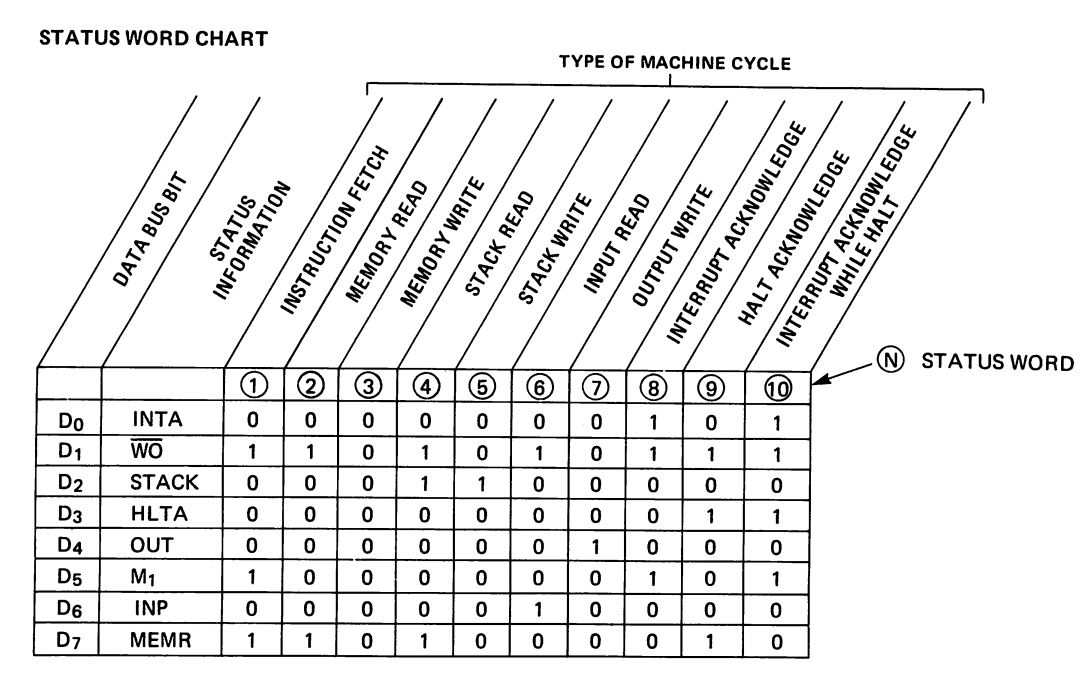
\includegraphics[width=15cm]{Bilder/Intel8080_DataLines}}

\newcommand{\Titel}{Konzeptionierung eines Simulators für 8-bit Prozessoren}
\newcommand{\ArtArbeit}{Studienarbeit}
\newcommand{\Abschluss}{Bachelor of Science}
\newcommand{\Studiengang}{Studiengang Informationstechnik}

\newcommand{\Ort}{Karlsruhe}


\newcommand{\imgSpaceBefore}{\\[0.2cm]}

%\newcommand{\Abgabedatum}{16.02.2021}


\begin{document}
\onehalfspacing
\pagenumbering{Roman}
	\begin{titlepage}
		{\DHBWLogoDeckblatt}\\[2cm]
		\begin{center}
			\vspace*{-2cm}
			{\Huge \Titel}\\[2cm]
			{\Huge \ArtArbeit}\\[2cm]
			{\Large \Abschluss}\\[0.5cm]
			{\large \Studiengang}\\[0.5cm]
			{\large an der}\\[0.5cm]
			{\large Dualen Hochschule Baden-Württemberg Karlsruhe}\\[0.5cm]
			{\large von}\\[0.5cm]
			{\large\bfseries \Autor}\\[1cm]
			{\large Abgabedatum \today}
			\vfill
		\end{center}
		\begin{tabular}{l@{\hspace{1cm}}l}
			Bearbeitungszeitraum & \Bearbeitungszeitraum \\
			Kurs & \Kurs \\
%			Ausbildungsfirma & \Ausbildungsfirma \\
			Betreuer der Ausbildungsfirma & \Betreuer \\
		\end{tabular}
	\end{titlepage}

\newpage

\thispagestyle{empty}
\begin{center}
\Large\bfseries Erklärung
\end{center}
\medskip
\noindent
Wir versichern hiermit, dass wir unsere \ArtArbeit \ mit
dem Thema: 
\begin{center}
	 \Titel \ 
\end{center}
selbstständig verfasst und keine anderen als die angegebenen Quellen und
Hilfsmittel benutzt haben. Wir versichern zudem, dass die eingereichte elektronische Fassung mit der
gedruckten Fassung übereinstimmt.

\vspace{3cm}
\noindent
\underline{\Ort, \today \hspace{9cm}}\\
%\hfill\underline{\hspace{6cm}}\\
Ort, Datum\hfill Unterschrift\hspace{4cm}

\newpage

\thispagestyle{empty}
\tableofcontents

\newpage

%\thispagestyle{empty}
\thispagestyle{plain}
\cleardoublepage
\addcontentsline{toc}{section}{\listfigurename}
\listoffigures

\addcontentsline{toc}{section}{\listtablename}
\listoftables

\addcontentsline{toc}{section}{Listings}
\lstlistoflistings

\newpage

%\thispagestyle{empty}
\thispagestyle{plain}
\cleardoublepage
\section*{Abkürzungsverzeichnis}
\addcontentsline{toc}{section}{Abkürzungsverzeichnis}
\textbf{ALU} - Arithmetic Logic Unit\\
\textbf{CISC} - Complex Instruction Set Computer\\
\textbf{GUI} - Graphical User Interface\\
\textbf{MISD} - Multiple-instruction stream single-data stream\\
\textbf{MIMD} - Multiple-instruction stream multiple-data stream\\
\textbf{RISC} - Reduced Instruction Set Computer\\
\textbf{SISD} - Single-instruction stream single-data stream\\
\textbf{SIMD} - Single-instruction stream multiple-data stream

\newpage
\pagenumbering{arabic}

%% Kopf und Fusszeilen==================================================== 
\pagestyle{scrheadings} % Seite mit Headern 

% loescht voreingestellte Stile 
\clearpairofpagestyles
%\clearscrheadings 
\clearmainofpairofpagestyles
%\clearscrplain 

% %%% Kopfzeile 
% einseitig: Bei einseitigem Layout, nur folgende Zeilen verwenden !!! 
%\ohead[] {
\includegraphics[height=0.5cm]{Logos/Firmenlogokopfzeile}}
\ihead[]{\leftmark} % links: Kapitel
%\chead[]{} % mitte: 

% %%% Fusszeile 
%\cfoot[]{} % mitte: 
\cfoot[\pagemark]{\pagemark} % rechts: Seitenzahl


% Angezeigte Abschnitte im Header 
\automark{section}  % Inhalt von [\rightmark]{\leftmark} 

\section{Einführung}
Dieses Kapitel befasst sich vorwiegend mit relevanten Grundlagen der Arbeit. Unter anderem wird das Ziel spezifiziert, elementare Aspekte der Arbeitsweise eines Prozessors werden erläutert und die verschiedenen Werkzeuge mit denen das Ziel realisiert wird werden aufgeführt.

\subsection{Ziel der Arbeit}
In dieser Arbeit soll ein Simulationsprogramm geschrieben werden, mit dem mehrere unterschiedliche 8-Bit Prozessoren simuliert werden können. Dazu sollen die Grundlegenden Eigenschaften in kurzen Lernprogrammen erläutert werden. Ebenfalls soll es eine interaktive Einweisung geben wie der Simulator verwendet werden kann.

\subsection{Zeitplan}
Platzhalter

\newpage

\subsection{Theoretische Grundlagen}
Als Vorbereitung für die Implementierung der verschiedenen Prozessoren werden einige allgemeingültige Architekturprinzipien eines Prozessors analysiert. 

\subsubsection{Architektur eines Prozessors}
Der fundamentale Aufbau eines Prozessors lässt sich in folgende Bausteine einteilen:\\
\textbf{Rechenwerk}\\
Das Rechenwerk ist die zentrale Einheit mit der eingehende Befehle verarbeitet werden. Es erhält Werte aus dem Speicher und führt damit in der ALU Operationen durch. Zum Rechenwerk dazugehörig sind auch Hilfsregister die beispielsweise als naher Zwischenspeicher fungieren.\\
\textbf{Steuerwerk}\\
Das Steuerwerk ist für die korrekte Abarbeitung von Befehlen zuständig. Es besteht aus dem Befehlsdekoder, dem Befehlszähler und einem Statusregister.\\
\textbf{Programmspeicher}\\
Der Programmspeicher eines Prozessors enthält die einzelnen Befehle, welche vom Befehlsdekoder dekodiert werden. Dabei wird der Befehl verwendet der an der vom Befehlszähler spezifizierten Stelle im Speicher steht.\\
\textbf{Ein-/Ausgabewerk}\\
Das Ein-/Ausgabewerk ist für die Kommunikation des Prozessors mit anderen Systemkomponenten verantwortlich.\\
\subsubsection{Befehlsformate}
Für einen Prozessor wird zwischen vier verschiedenen Befehlsformaten unterschieden. Diese beziehen sich auf die Anzahl der Adressen, welche der ALU bei Beginn einer Operation zur Verfügung gestellt werden.\\ \\
\textbf{Null-Adress-Anweisungen}\\
Vom Akkumulator (Stack) wird der Wert der zwei obersten Adressfeldern entnommen und die Operation wird auf diese ausgeführt. Der Speicherort des Ergebnisses ist ebenfalls vorbestimmt. Daher werden keine Adressen benötigt zum ausführen von Operationen.\\ \\
\textbf{Ein-Adress-Anweisungen}\\
Wie bei einer Null-Adress-Anweisung wird ein Wert aus dem Akkumulator entnommen. Ein zweiter Wert wird aus dem Speicher der übergebenen Adresse entnommen. Der Speicherort des Ergebnisses ist nach wie vor fest.\\
\textbf{Zwei-Adress-Anweisungen}\\
Für Zwei-Adress-Anweisungen ist es möglich eine Bezugsadresse für die Operanden anzugeben sowie eine Zieladresse, in der das Ergebnis der Operation gespeichert wird.\\ \\
\textbf{Drei-Adress-Anweisungen}\\
Drei-Adress-Anweisungen sind essentiell komplexere Zwei-Adress-Anweisungen. Eine der drei verfügbaren Adressen wird ebenfalls für die Zieladresse der Operation verwendet. Für das Beziehen der Operanden steht eine weitere Adresse zur Verfügung.\\

\subsubsection{CISC und RISC}
Von Andreas
komplettes Kapitel aus Buch \\
Ein Prozessor unterstützt immer nur eine gewisse Menge an Befehlen, diese werden Instruction Set genannt. Heutzutage gibt es zwei grundlegende Prozessorarchitekturen, Complex Instruction Set Computer (CISC) und Reduced Instruction Set Computer (RISC). Früher konnten Prozessoren genau einer dieser Gruppen zugeordnet werden, allerdings ist das bei den heutigen Prozessoren nicht mehr möglich, da sowohl RISC als auch CISC Befehle dem Prozessor zur Verfügung gestellt werden um die Vorteile von beiden zu haben.\\\\
Bei CISC-Prozessoren wird versucht soviel wie möglich in einem Befehl ausführen zu können. So gibt es viele verschieden Befehle, die auch unterschiedlich viel Zeit benötigen. Dadurch wird es aber auch möglich, komplexere Befehle direkt in der Hardware zu berechnen. Bei diesen Befehlen gibt es auch einige Adressierungsarten mehr als bei RISC-Prozessoren. Für vorbestimmte Aufgaben gibt es auch eigene Register, die nur dafür verwendet werden und davon auch nur wenige. Der Nachteil bei CISC-Prozessoren ist, dass die eigenen Befehle erst noch durch ein Mikroprogramm interpretiert werden müssen und dieses die komplexen Befehle in mehrere kleine Befehle aufteilen muss, welche erst dann vom Prozessor bearbeitet werden können. Dies kostet etwas mehr Zeit und verlangsamt die Ausführung. Die Mikroprogramme, die dafür verwendet werden, werden in einem kleinem Read-only Memory (ROM) gespeichert.\\\\
Bei RISC-Prozessoren wird versucht mit nur wenigen, kleinen Befehlen auszukommen. Diese sind wiederum sehr schnell, da sie meist fest verdrahtet sind, müssen aber mit anderen kombiniert werden um die Komplexität eines einzigen CISC-Befehls zu erreichen.  Im Gegensatz zu CISC-Prozessoren besitzen RISC-Prozessoren viele Register die frei verwendbar sind und nicht für speziellen Operationen bestimmt sind. Ebenso können die meisten Befehle in nur einem einzigen Arbeitsschritt ausgeführt werden.\\\\
Da bei CISC-Prozessoren mit nur einem Befehl viel berechnet werden kann, sind diese optimal für Übersetzer oder Interpreter geeignet. Bei der Entwicklung können dann einzelne komplexe Befehle verwendet werden anstatt von vielen kleinen. Jedoch können RISC-Prozessoren schneller Befehle ausführen, da:

\begin{itemize}
\item es nur wenige Befehle gibt und diese schnell decodiert werden können
\item die Befehle mithilfe von Pipelines effizienter abgearbeitet werden können
\item kein Mikroprogramm die einzelnen Befehle erst noch interpretieren muss
\end{itemize}
 

\subsubsection{Parallelität nach Flynn}
Von Andreas\\
1966 wurden von Micheal Flynn die folgenden vier Arten von Parallelisierung eingeführt [Flynn 949]:

\begin{itemize}
\item Single-instruction stream, single-data stream (SISD)
\item Single-instruction stream, multiple-data stream (SIMD)
\item Multiple-instruction stream, single-data stream (MISD)
\item Multiple-instruction stream, multiple-data stream (MIMD)
\end{itemize}
\noindent
\textbf{SISD}\\
Diese Beschreibung trifft auf die einfachen Einprozessorsysteme zu. Dabei kann immer nur eine Operation gleichzeitig ausgeführt werden und diese werden in nur einer möglichen Reihenfolge aus einem Daten-Strom abgearbeitet.\\
\noindent
\textbf{SIMD}\\
Bei SIMD werden Pipelines eingesetzt, die es ermöglichen mehrere korrekte Abfolgen von Programmbefehlen auszuführen. So können unterschiedliche Programme in sich selber in der richtigen Reihenfolge aber mit anderen Programmen abwechselnd ausgeführt werden.\\
\noindent
\textbf{MISD}\\
Diese Variante scheint auf Anhieb keinen effizienten Nutzen zu besitzen, da mehrere Prozessoren alle die gleichen Befehle ausführen, die aus einem Daten-Strom stammen. Dies kann aber dazu verwendet werden um die Korrektheit durch Redundanzen zu bestätigen. \\
\noindent
\textbf{MIMD}\\
Diese Architektur verwendet mehrere Prozessoren und mehrere Daten-Ströme. Heutzutage ist dies unter dem Begriff Mehrprozessorsysteme bekannt. So werden für jeden einzelnen Prozessor ein Daten-Strom erzeugt der unabhängig von den anderen Prozessoren arbeiten kann. Dabei ist es für die Prozessoren aber trotzdem möglich die Daten der anderen Prozessoren zu nutzen. Nur durch MIMD oder MISD, also die Ausführung mit mehreren unabhängigen Prozessoren, ist es möglich Programme tatsächlich parallel ablaufen zu lassen. Mit SISD oder SIMD sind nur quasi parallele Ausführungen möglich.\\

\subsection{Instruction Sets}
Von Andreas\\
Die meisten Prozessoren besitzen Befehle aus den folgenden fünf Gruppen:
\begin{itemize}
\item Daten Transfer Gruppe
\item Arithmetik Gruppe
\item Logische Gruppe
\item Verzweigungs Gruppe
\item Stapel, Ein- Ausgänge und Maschinen Kontroll- Gruppe
\end{itemize}\noindent
Die Befehle der Daten Transfer Gruppe bewegen Daten zwischen Registern und/oder Speicher wie zum Beispiel mit den MOVE Befehlen. In der Arithmetik Gruppe werden, wie der Name schon sagt, Befehle mit arithmetische Operationen wie Addition verwendet. In der Logischen Gruppen werden Operation wie das logische Oder verwendet. In der Zweig Gruppe gibt es die Befehle, welche den Standardmäßigen Programmfluss ändern und das Programm nicht zwangsläufig in der nächsten Zeile fortgesetzt wird wie bei bedingten Sprüngen. In der letzten Gruppe liegen die Befehle, die Eingänge und Ausgänge beachten oder den Stack bearbeiten. [Intel 8080 S.46 (4-1)]
\\

\newpage

\section{Projektplanung}
Platzhalter

\subsection{Auswahl geeigneter Varianten}
Vor der Implementierung des Simulators müssen einer oder mehrere geeignete Prozessoren ausgewählt werden. In den nachfolgenden Kapiteln werden einige potenzielle Kandidaten näher analysiert und beschrieben.

\subsection{Intel 8080}
Der Intel8080 bietet ein breites Spektrum an Befehlen und wäre auch repräsentativ für einen der ersten großen, kommerziell erfolgreichen Prozessoren. Aufgrund der überschaubaren Komplexität besteht auch die Möglichkeit diesen in einem größeren Unmfang zu simulieren.

\subsubsection{Register}
\label{RegisterSection}
Von Andreas\\ \noindent
Der Intel 8080 besitzt ein SRAM Array mit 16-bit Register. Darin enthalten sind der Programm Counter mit 16-bit und der Stack Pointer mit 16-bit. Dazu gibt es noch acht weitere 8-bit Register. Diese können entweder alleine oder zusammen mit einem anderen 8-bit Register als ein 16-bit Register verwendet werden. Dabei gibt es aber nur die fest vorgegebenen Kombinationen. Das B- und C-Register, das D- und E-Register, das H- und L- Register und die temporären W- und Z- Register. Die W- und Z-Register können nicht vom Programmierer verwendet werden und dienen nur zur internen Ausführung von Befehlen. 
Über einen Multiplexer ist es möglich acht Bit auf den internen Adressbus zu schreiben oder von dort zu lesen. \textbf{Über das Adress-Latch oder den Incrementer/Decrementer-Circuit ist es möglich 16-Bit aus den Registern weiterzuleiten. Von dort aus können die Werte dann in den Adress-Puffer geschrieben werden.} [Intel 8080 S16 (2-2)]


\subsubsection{Befehle}
Von Andreas\\ \noindent
Der Intel 8080 ist in der Lage Befehle, die aus einem, zwei oder drei Bytes bestehen, auszuführen. Dabei gibt das erste Byte immer den Opcode oder Operation Code an. In Byte zwei und drei werden nur Daten oder Adressen gespeichert. Dabei werden die zwei Byte großen Adressen so gespeichert, dass das niederwertige Byte vor dem höherwertigem gespeichert wird. Die Adressen können dabei über vier verschiedene Modi verwendet werden.
\begin{itemize}
\item Direct
\item Register
\item Register Indirect
\item Immediate
\end{itemize}\noindent
Bei "Direkt"' wird der Wert in dem Speicher mit der angegebenen Adresse verwendet. Hier werden das Low-Byte im zweiten und das High-Byte im dritten Byte gespeichert. Bei "Register"' wird auf ein oder zwei Register verwiesen und verhält sich wie bei Direkt. Bei "Register Indirect"' wird der Wert aus der Adresse aus dem zweiten und dritten Byte des Befehls gelesen. Dieser Wert wird als Adresse verarbeitet und erst der Wert aus dieser Adresse ist der zu verwendete Wert. Bei [TODO]\glqq Immediate\grqq steht 
im zweiten und/oder dritten Byte ein Wert mit dem gearbeitet wird (Lowbyte im zweiten Byte). [Intel 8080 S.47 (4-2)]
\\ \noindent
Bei Interrupts und Branch Befehlen gibt es nur den "Direct"' und "Register indirect"' Modus [Intel 8080 S.47 (4-2)]. 
\\ \noindent
Der Prozessor besitzt fünf Condition Flags. Das Zero flag, das angibt ob das Ergebnis eines Befehls den Wert 0 hatte. Das Sign flag, welches angibt ob Bit 8, das Most Signifikant-Bit, des letzten Ergebnisses den Wert 1 hat. Das Paritäts flag, welches gesetzt ist, wenn das letzte Ergebnis einen Modulo 2 Wert von 0 hat, also der Wert gerade ist. Das Carry flag, das einen Übertrag bei einer Addition oder einen Abzug bei einer Subtraktion oder Vergleich anzeigt und noch das Auxiliary Carry flag, welches ebenfalls einen Übertrag oder Abzug anzeigt aber zwischen dem vierten (Bit 3) und fünften Bit (Bit 4). [Intel 8080 S.47f (4-2)]
\\

\subsubsection{Data Transfer Group}
Für den Prozessor sind 13 Befehle aus dieser Gruppe bekannt. Bei keinem dieser Befehle werden die Condition Flags gesetzt oder zurückgesetzt.

\begin{multicols}{2}
\begin{itemize}
\item Move Register
\item Move from Memory
\item Move to Memory
\item Move immediate
\item Move to Memory Immediate
\item Load register pair immediate
\item Load Accumulator direct
\item Store Accumulator direct
\item Load H and L direct
\item Store H and L direct
\item Load Acumulator indirect
\item Store Accumulator indirect
\item Exchange H and L with D and E
\end{itemize}
\end{multicols}


\subsubsection{Arithmetic Group}
20 Befehle
Unless indicated otherwise, all instructions in this
group affect the Zero, Sign, Parity, Carry, and Auxiliary
Carry flags accord ing to the standard rules.
All subtraction operations are performed via two's
complement arithmetic and set the carry flag to one to indicate a borrow and clear it to indicate no borrow

\begin{multicols}{2}
\begin{itemize}
\item Add Register
\item Add Memory
\item Add immediate
\item Add Register with carry
\item Add Memory with carry
\item Add immediate with carry
\item Sustract Register
\item Subtract Memory
\item Subtract immediate
\item Subtract Register with borrow
\item Subtract Memory with borrow
\item Subtract immediate with borrow
\item Increment Register
\item Increment Memory
\item Decrement Register
\item Decrement Memory
\item Increment register pair
\item Decrement register pair
\item Add register pair to H and L
\item Decimal Adjust Accumulator
\end{itemize}
\end{multicols}

\subsubsection{Logical Group}
19 Befehle
Unless indicated otherwise, all instructions in this
group affect the Zero, Sign, Parity, Auxiliary Carry, and
Carry flags according to the standard rules

\begin{multicols}{2}
\begin{itemize}
\item AND Register
\item AND Memory
\item AND immediate
\item Exclusive OR Register
\item Exclusive OR Memory
\item Exclusive OR immediate
\item OR Register
\item OR Memory
\item OR immediate
\item Compare Register
\item Compare Memory
\item Compare immediate
\item Rotate left
\item Rotate right
\item Rotate left through Carry
\item Rotate right through Carry
\item Complement Accumulator
\item Complement Carry
\item Set Carry
\end{itemize}
\end{multicols}


\subsubsection{Branch Group}
8 Befehle
Flags are not affected

\begin{itemize}
\item Jump
\item Conditional Jump
\item Call
\item Conditional Call
\item Return
\item Conditional Return
\item Restart
\item Jump H and L indirect - move H and L to PC
\end{itemize}

\subsubsection{Stack, I/O and Machine Control Group}
12  Befehle
Unless otherwise specified, condition flags are not
affected by any instructions in this group

\begin{multicols}{2}
\begin{itemize}
\item Push
\item Push Processor status word
\item Pop
\item Pop processor status word
\item Exchange stack top with H and L
\item Move HL to SP
\item Input
\item Output
\item Enable Interrupts
\item Disable Interrupts
\item Halt
\item No op
\end{itemize}
\end{multicols}


\subsubsection{Maschinenzyklen und Typen}
Jeder Befehl oder Befehlszyklus benötigt mindestens einen und maximal fünf Maschinenzyklen zum kompletten Ausführen des Befehls. Dabei kann jeder Befehl aus mehreren Typen bestehen, wobei der erste immer ein Fetch-Befehlstyp ist. Die existierenden Befehlstypen sind:

\begin{itemize}
\item Fetch
\item Memory Read
\item Memory Write
\item Stack Read
\item Stack Write
\item Input
\item Output
\item Interrupt
\item Halt
\item Halt Interrupt
\end{itemize}\noindent
Jeder Maschinenzyklus besteht nochmal aus drei bis fünf Zuständen. So kann ein Befehl insgesamt zwischen vier und achtzehn Zuständen andauern.
In dem ersten Zustand jedes Maschinenzykluses wird immer der Befehlstyp während des SYNC-Taktes kodiert. Die folgende Abbildung zeigt, wie die Befehlstypen über die \textbf{Data Lines} kodiert werden. [Intel 8080 S17ff. 2-3]
\imgSpaceBefore

\begin{figure}[h]
\caption{Kodierung der Befehlstypen beim SYNC Takt}
\centering
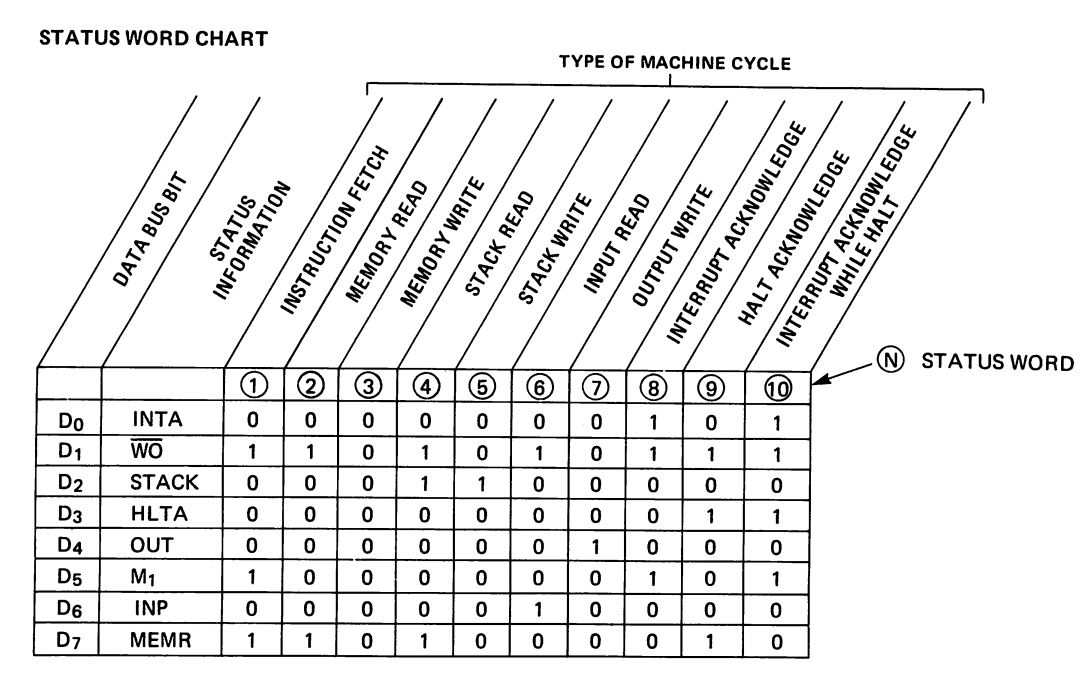
\includegraphics[width=15cm]{Bilder/Intel8080_DataLines}
\label{fig:Intel8080_DataLines}
\end{figure}


\subsection{Beispielprozessor 2}
Fällt vermutlich weg
\subsection{Beispielprozessor 3 ...}
s.o.\\
Kommentar: Ein weiterer Prozessor sollte zumindest in Ansätzen analysiert werden.

\newpage

\section{Umsetzung}
In diesem Kapitel wird darauf eingegangen wie die in Kapitel 2 erarbeitete Analyse der ausgewählten Prozessoren implementiert wird.
\subsection{Abstraktion der Architektur}
Es ist vorgesehen, dass der Prozessor in verschiedene Unterklassen aufgeteilt wird. Dabei ist vorgesehen das dies in einer Art Stern-Struktur aufgebaut wird, das heißt die verschiedenen Bestandteile des Prozessors sollen alle mit einer zentralen Klasse interagieren, aber nicht untereinander.
\subsubsection{Prozessor}
Die Prozessor-Klasse soll die zentrale Einheit des Simulators sein. Über diese sollen sowohl Anfragen über Informationen vorgenommen werden, zum Beispiel um diese in der Benutzeroberfläche anzuzeigen, als auch Instruktionen an den Prozessor als ganzes gesendet werden. Dabei ist zu unterscheiden zwischen zwei Arten von Anfragen, gültige und ungültige. Gemeint ist sind damit Anfragen in einem echten Prozessor zulässig wären, beispielsweise einen externen Bus zu befüllen oder die nächste Anweisung auszuführen, und Anfragen die unzulässig wären, wie den Programmzähler manuell zu setzen.
\subsubsection{ALU}
Die ALU soll die Bearbeitung logischer Operationen im Prozessor simulieren. Sinn ist dabei ein möglichst genaues Bild jedes Zustandes des Prozessors darzustellen, statt beispielsweise solche Operationen einfach manuell in der Prozessor-Klasse abzuarbeiten.
\subsubsection{Register}
Die Register-Klasse soll ähnlich wie die ALU den Zugriff möglichst realitätsgetreu simulieren. Dabei sollen Methoden die den Zugriff regeln ähnlich aufgebaut werden wie es im echten Prozessor möglich wäre.
\subsubsection{Peripherie}
Mit der Peripherie soll alles abgedeckt werden was nicht Teil der zentralen Bestandteile ist, also der Register oder der ALU. Dazu zählt zum Beispiel ein externer Datenbus oder Schnittstellen für bspw. Taktsignal o.ä.
\subsection{Möglichkeiten des Simulation}
Um einen Ablauf für die Simulation festzulegen muss erst bestimmt welche Parameter eingestellt, welche Optionen verändert und welche Operationen im Simulator durchgeführt werden können.
\subsection{Ablauf der Simulation}
\subsection{Aufbau der GUI}
\subsection{Tutorials}

\newpage

\section{Implementierung}
Mit diesem Simulator soll es möglich sein Assembler Code in ein Textfeld einzugeben und diesen dann ausführen zu können. Damit dies möglich ist muss der Assembler Code erst erstellt werden. Dies wird mit einem einfachen Assembler aus dem Internet gemacht. Dieser erstellt aus dem Source Code (.asm) eine .com-Datei, woraus die Befehle byteweise ausgelesen werden können. Manche Befehle verwenden aber auch mehr als ein Byte. Zusätzlich dazu wird noch eine Datei (.sym) erstellt, die die Lables/Sprungmarken abspeichert.

Unser eigentlicher Simulator verendet nur die .com-Dateien. Aus dieser Datei wird als aller ersten nur ein Byte gelesen. Mithilfe des ersten Bytes wird analysiert um welchen Befehl es sich handelt. Je nach Befehl werden noch weitere Bytes eingelesen, die für den eigentlichen Befehl gebraucht werden. Somit werden nie zu wenig oder zu viele Bytes gelesen. Aus der Datei werden immer anhand des Programmzählers die nächsten Bytes ausgelesen. In unserem Programm wurde das so implementiert, dass direkt beim lesen eines Bytes der Programmzähler um eins erhöht wird. Damit muss aber darauf geachtet werden, dass Bytes nicht mehrfach gelesen werden sollen, da, zum einen zwei unterschiedliche Werte gelesen werden und zum anderen der Programmzähler um ein weiteres Mal erhäht wird und somit ein Byte überspringt.
\imgSpaceBefore

\begin{figure}[h]
\caption{Implementierung des Lesens eines Bytes}
\centering
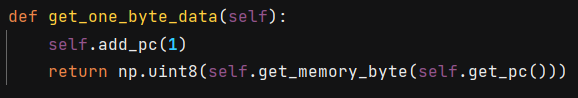
\includegraphics[width=15cm]{Bilder/GetOneByteData}
\label{fig:GetOneByteData}
\end{figure}

Nachdem erkannt wurde um welchen Befehl es sich handelt werden, werden zwei Arten unterschieden. Befehle wie Sprungbefehle, die die ALU nicht benötigen und Befehle wie Additionen, die die ALU verwenden. Der Simulator besteht hauptsächlich aus drei Klassen:

\begin{itemize}
\item Dem Prozessor (Intel8080.py)
\item Der ALU (Intel8080\_ALU.py)
\item Die Register (Intel8080\_Registers.py)
\end{itemize} 

Die Befehle, die die ALU nicht verwenden wurden in in der Intel8080.py implementiert. Die anderen entsprechend in der ALU. 


\subsection{Erkennen eines Befehls aus einem Byte}
Nachdem der Assembler Code in das Textfeld eingegeben wurde und 
[TODO] auf \glqq Play\grqq gedrückt wurde, 
wird der Assembler Code compiliert. Um damit später besser arbeiten zu können, werden diese Werte direkt in einem Array für den Prozessor gespeichert. In jeder Zelle steht dann genau ein Byte. 

Um einen Befehl analysieren zu können muss zunächst ein Byte aus dem Array gelesen werden. Dieser Wert wird mehrfach mit vielen Hexadezimalen Werten verglichen. Anhand der Dokumentation des Intel 8080 werden somit alle Befehle unterschieden. 
[TODO] Wie in  Abbildung \ref{fig:ReadInstruction} zu sehen ist, wird der Befehl \glqq Add Immediate to A with carry (ACI)\grqq mit dem Wert 0xCE beschrieben.  
Bei vielen Befehlen wie ACI wird auf genau einen Wert geprüft. Ebenfalls ist in Abbildung \ref{fig:ReadInstruction} zu sehen, dass der Befehl \glqq Add Memory to A with carry (ADC)\grqq nicht so einfach verglichen wird. Bei diesem Befehl werden in den letzten drei Bits des Befehlsbytes das 8-Bit-Register kodiert, welches verwendet werden soll. Deshalb wird die Instruction Variable zuerst mit dem Wert 0xF8 bitweise verundet, damit die letzten drei Bit ignoriert werden. Somit werden alle Bitkombinationen erkannt, bei der die ersten 5 Byte mit dem Wert 0x88 übereinstimmen. 
\imgSpaceBefore

\begin{figure}[h]
\caption{Implementierung des Lesens des ersten Bytes eines Befehls}
\centering
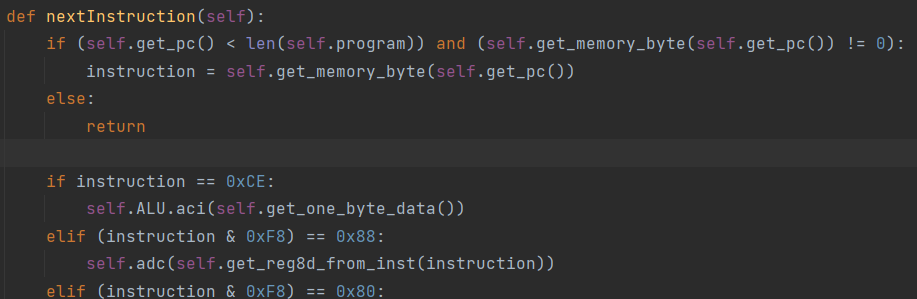
\includegraphics[width=15cm]{Bilder/ReadInstruction}
\label{fig:ReadInstruction}
\end{figure}

Bei einigen anderen Befehlen wird diese Mechanik genauso verwendet. Es gibt aber auch Befehle, da werden die 8-Bit-Register in den Bits drei bis fünf codiert. Ebenso gibt es Befehlen, welche auch 16-Bit-Register verwenden z.B.
[TODO] \glqq Load Immediate register/stack pointer (LXI)\grqq 
. Wie auf Seite \pageref{RegisterSection} beschrieben, können auch zwei 8-Bit-Register zu einem 16-Bit-Register zusammen geschlossen werden und damit verwendet werden. Insgesamt gibt es davon drei Kombinationen. In diesen Befehlen werden diese Register mit zwei Bit kodiert. Damit gibt es noch eine Bitkombination, mit der noch ein weiteres Register verwendet werden kann. Mit der vierten noch übrig gebliebenen Kombination wird der Stackpointer als 16-Bit-Register verwendet werden. 




\subsection{Mehrfach verwendete Methoden}

Der Intel 8080 kennt mehrere Befehle, die sowohl eine direkte als auch eine indirekte Variante. Der Unterschied bei diesen Varianten sind nur, dass die Werte, mit denen gerechnet wird, von unterschiedliche Stellen geladen werden. Aus diesem Grund greifen beide Befehle im Hintergrund auf die gleichen Methoden zu. Somit ist sicher gestellt, dass falls nochmal etwas an der Implementierung geändert werden soll, das nur an einer Stelle gemach werden muss.

Ein Beispiel dafür ist die \glqq Subtract register/immediate from A with borrow (SBB/SBI)\grqq. Es gibt für beide Mnemonics eine Methode in der Intel8080-Klasse aber die Methode von SBB leitet später in der ALU-Klasse nur noch auf die SBI-Methode weiter.
\imgSpaceBefore

\begin{figure}[h]
\caption{Zugrunde liegende Implementierung von SBB und SBI}
\centering
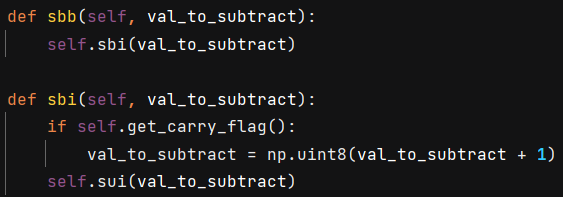
\includegraphics[width=15cm]{Bilder/DoubleUsedMethodSubtract}
\label{fig:DoubleUsedMethodSubtract}
\end{figure}

Zu Beginn der Analyse der Befehle, wird für SBI direkt das nächste Byte gelesen und damit die Methode SBI in der ALU-Klasse aufgerufen. Für SBB wird zunächst in der Intel8080-Klasse noch der Wert aus dem Speicher gelesen, da dies von der ALU nicht möglich ist. Mit dem gelesenem Wert wird dann in der ALU-Klasse die SBB-Methode aufgerufen. Diese leitet innnerhalb der Klasse aber nur noch auf die SBI Methode weiter.
\\

Ähnliches wird auch bei bei den Sprungbefehlen gemacht. Dort gibt es mehrere Varianten, die aber nur auf unterschiedliche Flags reagieren. Deshalb wurde auch dort eine zugrundeliegende Methode geschrieben, auf die alle anderen verweisen. So wird nur für die spezifische Varianten, das verwendete Flag weitergegeben.  Abbildung \ref{fig:JumpVariants} zeigt wie bei den Jump on Carry Befehl vorgegangen wird. So ruft die jc-Methode, die jump\-on-Methode mit dem Carry-Flag auf. In der jump\_on-Methode werden immer die nächsten zwei Bytes gelesen, die auf die Programmstelle weisen, auf die gesprungen werden soll. Nur sofern das übergebene Flag gesetzt ist wird der Sprung ausgeführt. Wenn nicht wird das Programm normal weitergeführt.
\imgSpaceBefore

\begin{figure}[h]
\caption{Implementierung der Sprungbefehle}
\centering
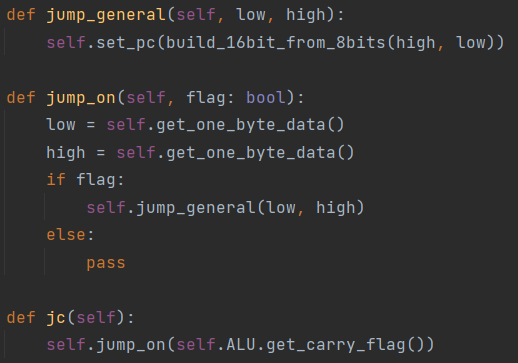
\includegraphics[width=15cm]{Bilder/JumpVariants}
\label{fig:JumpVariants}
\end{figure}

\newpage

\section{Fazit und Ausblick}
Platzhalter

\newpage


\addcontentsline{toc}{section}{Literatur}
\begin{thebibliography}{9}
\bibitem{Beispiel}
Google: \url{https://www.google.com}
\bibitem{Grundlagen der Informatik}
Grundlagen der Informatik: Herold, Lurz, Wohlrab und Hopf; 3. aktualisierte Auflage (2017), Pearson
\bibitem{Adressformate}Instruction formats: \url{https://www.geeksforgeeks.org/computer-organization-instruction-formats-zero-one-two-three-address-instruction/}, zuletzt abgerufen: 25.12.2021
\end{thebibliography}



%\newpage
%\thispagestyle{empty}
%
%\section*{Anhang}
%\addcontentsline{toc}{section}{Anhang}


\end{document}